Пример оформления четырёх иллюстраций в одном текстово-графическом объекте приведён на \firef{fig:spbpu_sc-four-photos}. Это возможно благодаря использованию пакета \verb|subcaption|.

\begin{figure}[ht]
	\adjustbox{minipage=1.3em,valign=t}{\subcaption{}\label{fig:spbpu_sc-a}}%
	\begin{subfigure}[t]{\dimexpr.5\linewidth-1.3em\relax}
		\centering
		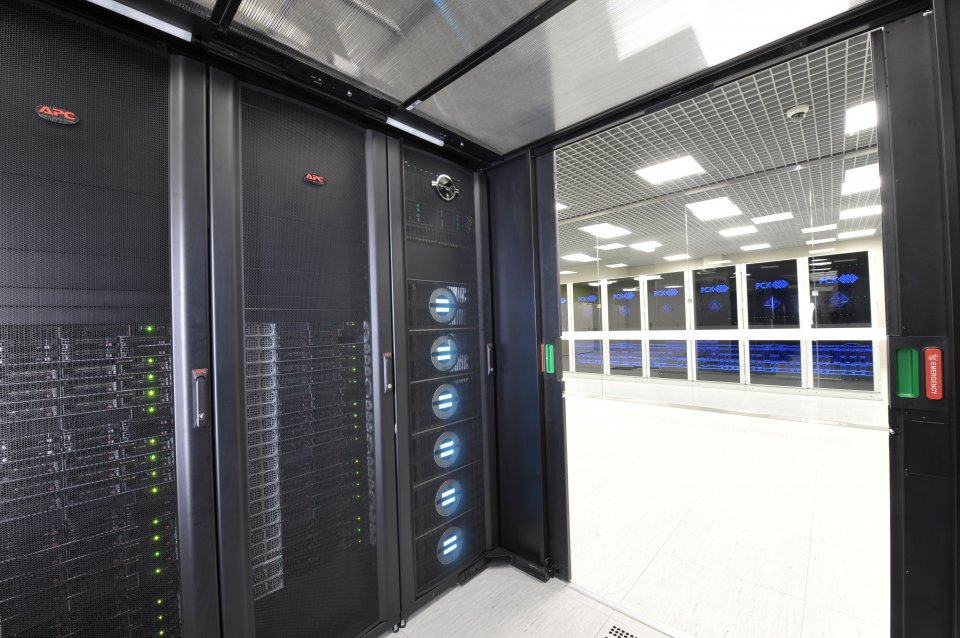
\includegraphics[width=.95\linewidth,valign=t]{my_folder/images/spbpu_sc_system}
	\end{subfigure}
\hfill %выровнять по ширине
	\adjustbox{minipage=1.3em,valign=t}{\subcaption{}\label{fig:spbpu_sc-b}}%
	\begin{subfigure}[t]{\dimexpr.5\linewidth-1.3em\relax}
		\centering
		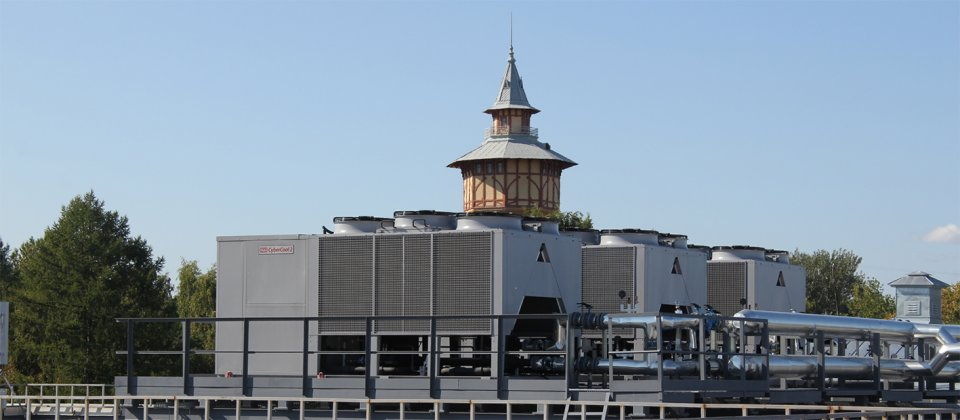
\includegraphics[width=.95\linewidth,valign=t]{my_folder/images/spbpu_sc_refr}
	\end{subfigure}
\\[20pt]
	\adjustbox{minipage=1.3em,valign=t}{\subcaption{}\label{fig:spbpu_sc-c}}%
\begin{subfigure}[t]{\dimexpr.5\linewidth-1.3em\relax}
	\centering
	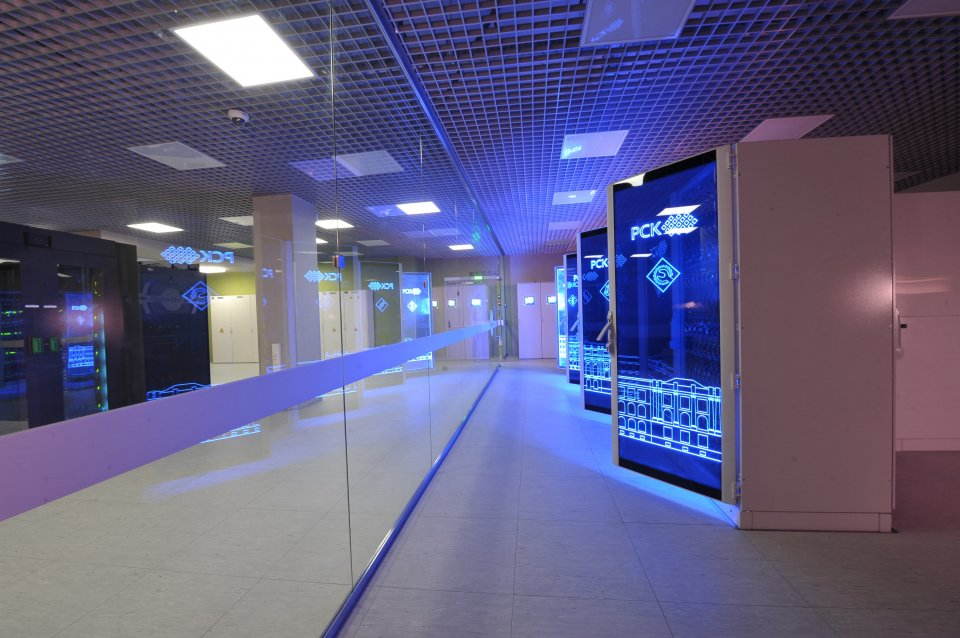
\includegraphics[width=.95\linewidth,valign=t]{my_folder/images/spbpu_sc_hall}
\end{subfigure}%
\hfill %выровнять по ширине
\adjustbox{minipage=1.3em,valign=t}{\subcaption{}\label{fig:spbpu_sc-d}}%
\begin{subfigure}[t]{\dimexpr.5\linewidth-1.3em\relax}
	\centering
	
\includegraphics[width=.95\linewidth,valign=t]{my_folder/images/spbpu_sc_box}
\end{subfigure}
\captionsetup{justification=centering} %центрировать
\caption{Фотографии суперкомпьютерного центра СПбПУ \cite{spbpu-gallery}: {\itshape a} --- система хранения данных и узлы NUMA-вычислителя; {\itshape b} --- холодильные машины на крыше научно-исследовательского корпуса; {\itshape c} --- машинный зал; {\itshape d} --- элементы вычислительных устройств} 
\label{fig:spbpu_sc-four-photos}
\end{figure}

Далее можно ссылаться на составные части данного рисунка как на самостоятельные объекты: \firef{fig:spbpu_sc-a}, \firef{fig:spbpu_sc-b}, \firef{fig:spbpu_sc-c}, \firef{fig:spbpu_sc-d} или на три из четырёх изображений одновременно: рис.\labelcref{fig:spbpu_sc-a,fig:spbpu_sc-b,fig:spbpu_sc-c}.